% -----------------------------------------------
% Template for ISMIR 2013
% (based on earlier ISMIR templates)
% -----------------------------------------------

\documentclass{article}
\usepackage[utf8]{inputenc}
\usepackage{ismir2013,amsmath,cite}
\usepackage{graphicx}

% For Graphs
\usepackage{tikz}
\usetikzlibrary{shapes,arrows}
\usetikzlibrary{calc}
\usepackage{caption}

%For Tables
\usepackage{booktabs}
\usepackage{graphicx}
%\usepackage[showframe]{geometry}

% Title.
% ------
\title{CSC 475 Final Project: Automatic Chord Estimation (Design Specification and Progress Report)}

% Three addresses
% --------------
\threeauthors
{Lee Gauthier} {\tt lgauthie@uvic.ca}
{Robert Janzen} {\tt rjanzen@uvic.ca}
{Sondra Moyls} {\tt smoyls@uvic.ca}

\begin{document}
%
\maketitle
%


\section{Abstract}\label{sec:desoutline}
This project aims to investigate and evaluate some of the current most popular
strategies for automatic chord estimation. We present a simple HMM-based model 
for detecting chords form audio signals using chroma vectors. We also evaluate the 
effectiveness of Harmonic/Percussive Sound Separation (HPSS) as a preprossing step by comparing
the results of an unaltered data set to the results of a dataset that has undergone
HPSS preprocessing. Our results show ....EDIT ME.... We concluse by discussing future improvements
to our model.

\section{Introduction}\label{sec:intro}

Chords describe the harmonic content of a piece of music. Automatic estimation of chords
has many applications in music information retreival and music annotation. For example,
automatic chord estimation may be used to inference genre and emotional content 
(minor, sad; major, happy) of a piece, or to identify songs of similar form. 
They have also been used successfully in detecting cover-songs \cite{Papadopoulos:18}.

Automatic chord detection has been a MIREX task since 2008, and has since seen increased
improvement, with submissions in 2012 surpassing 72 percent accuracy on unseen data 
\cite{McVicar:00}. Hidden Markov Models have been used successfully in a number of 
automatic chord estimation models, including \cite{Ueda:01} \cite{Lee:15} \cite{Ueda:19}
and \cite{Papadopoulos:18}.

...EDIT: Write more about previous papers that used HPSS, and beat synchronous extraction
when you are less a sleepy bear ...


\section{Overview}\label{sec:approch}

For this project we will use the annotated Billboard 100 data set. This data
set includes audio files for approximately 650 audio files from the Billboard
top 100 chart between the years 1958 and 1991. Each song also includes beat by
beat chord annotation \cite{Burgoyne:07}. The chords are labeled as either maj,
min, aug, dim, sus2, sus4, X, or N, where X and N imply no chord is present or
detected. A distinction is made between enharmonic labels (for example both
G\# and Ab occur in the annotations), for a total of 128 states. 
For the scope of this project we will not try to classify inverted
chords and 7th chords independently, and instead will classify them as one of
the previously mentioned classes.

\begin{figure}
\begin{center}
	\resizebox{0.4\textwidth}{!}{%
	\begin{tabular}{l c}
	\toprule
	 Original Chord Labels        & Treated As   \\ \midrule
	 Maj, Aug, sus4, sus2      & Maj           \\
	 min, dim                        & min           \\
	\bottomrule
	\end{tabular}
	}
\caption{Chord Labels}
\label{fig:chordlabs}
\end{center}
\end{figure}

We use two sets of audio data, one unprocessed, and one preprocessed by
performing harmonic percussive source separation (HPSS). It has been noted that 
applying this pre processing step can greatly improve chord estimation accuracy \cite{Reed:09}. 
In a spectrogram the harmonic components of a musical signal have 
a stable pitch and form parallel ridges along the time axis. Transient sounds distribute 
their frequency content across the entire spectrum and occur during short time frames, 
which can be seen as spikes in the frequency axis. The end product of HPSS is two signals, 
one with mostly harmonic content, the other with percussive sounds which is obtained by 
complementary diffusion on the spectrogram.

Each audio file is mixed to mono to reduce processing time. Then Chorma vector extraction is 
performed on the two auto datasets at intervals corresponding to the beat information in the 
annotated data. Each chroma vector is a real valued vector which contains the salience of each 
of the pitch classes (C, C\#.... B) for a given time window.

After extracting the chroma vectors for each song in the data set, 63 of the tracks are randomly
chosen using the random function in python and kept as testing data. The rest of the data set
is used to train our HMM model. Hidden Markov Models (HMMs) are currently the most common method for 
predicting chord labels, and also produce high accuracy scores. Previous use of
preprocessing of input data has also been explored and is summarized in \cite{McVicar:00}.

To create a supervised model, the transition matrix, prior, and mean and convariance of the 
vectors is created and run through functions available through
SciKit Learn for convenient training and testing. A full overview of our
proposed model can be seen in Figure \ref{fig:overview}.

% Define block style
\tikzstyle{block} = [rectangle, draw, fill=blue!20,
    text width=7em, text centered, rounded corners, minimum height=4em]
\tikzstyle{line} = [draw, -latex']

\begin{figure}
\begin{tikzpicture}[node distance=3cm]
    % Place nodes
    \node [block] (init) {Billboard Data Set};
    \node [block, below left of= init] (chordlabel) {Labeled Chords By Beat (.txt)};
    \node [block, below right of= init] (audio) {Audio (.wav)};
    \node [block, below of= chordlabel] (chordname) {Chord Names at Beat Times};
    \node [block, below of= audio] (chroma) {12-bin chroma features};
    \coordinate (Middle) at ($(chordlabel)!0.5!(chroma)$);
    \node [block, below of  =Middle, yshift=-1cm] (hmm) {HMM};
    \node [below of  =Middle] (train) {Training};
    % Draw edges
    \path [line] (init) -- (audio);
    \path [line] (init) -- (chordlabel);
    \path [line] (chordlabel) -- node {Analyze Groud Truth} (chordname);
    \path [line] (audio) -- node {Analyze Chroma} (chroma);
    \path [line] (chroma) -- (hmm);
    \path [line] (chordname) -- (hmm);

\end{tikzpicture}
\caption{System Overview}
\label{fig:overview}
\end{figure}

\section{Model}

\subsection{PreProcessing}
Harmonic percussive source separation was completed using the Librosa package created by Brian McFee.
The package is written in Python and uses scikit to perform two dimensional median filtering. The
STFT and ISTFT are both custom implementations. The median filters operates by replacing a given sample
in a signal by the median of the signal values in a window around the sample \cite{FitzGerald:11}. The input
audio is mixed to mono and the original 44.1 kHz sampling rate is used. 

$$y(n) = median \left \{x(n-k:n+k),l = (l-2)/2  \right \}$$

Each spectrogram is then translated back to the time domain where it can then be run through the
feature extraction system.

\begin{figure}
   \centering
    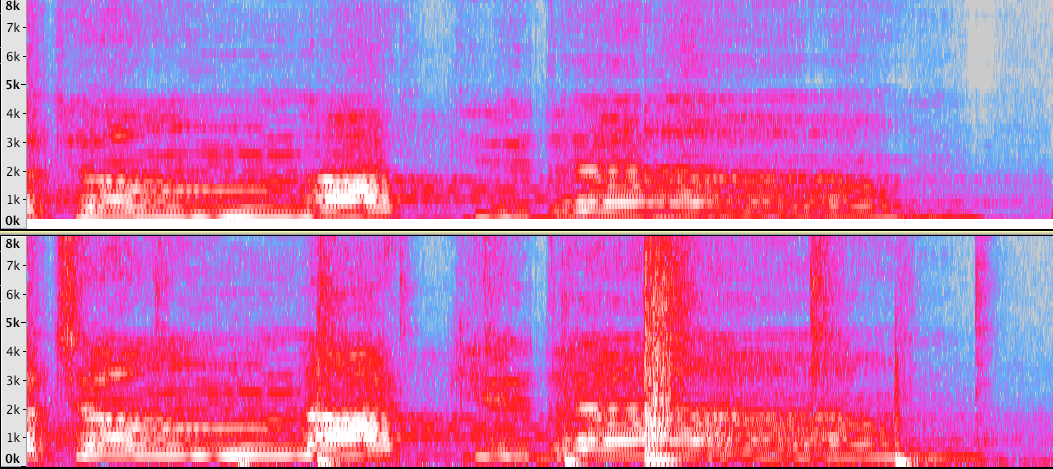
\includegraphics[width=0.5\textwidth]{hpssspec.png}
   \caption{Top: Harmonic result of HPSS, Bottom: Original Signal}
   \label{fig:HPSS}
\end{figure}


\begin{figure*}
	\resizebox{\textwidth}{!}{%
	\begin{tabular}{l c c c c}
	\toprule
	 & 64 Test Set Avg             & All Songs Test Set Avg & All Songs Test Set Max &  \\ \midrule
	Non-Processed                  & 1.0\% & 1.0\% & 20.7\%  &  \\
	HPSS                                  & 1.5\% & 1.0\% & 19.9\%  &  \\
	Non-Processed - 2 Iter      & 3.2\% & 2.9\% & 44.7\%  &  \\
	HPSS - 2 Iter                      & 3.7\% & 3.4\% & 60.5\%  &  \\
	Non-Processed - 10 Iter    & 3.5\% & 3.2\% & 38.9\%  &  \\
	HPSS - 10 Iter                    & 4.1\% & 4.1\% & 36.5\%  &  \\
	Non-Processed - 100 Iter  & 4.2\% & 3.9\% & 17.1\%  &  \\
	HPSS - 100 Iter                  & 5.1\% & 4.6\% & 18.0\%  &  \\
	100 Songs - 500 Iter         & 5.5\% & 5.3\% & 20.1\%  &  \\
	HPSS 100 Songs - 500 Iter & 6.2\% & 6.4\% & 25.8\%  &  \\
	\bottomrule
	\end{tabular}
	}
\caption{Results Table}
\label{fig:resulttable}
\end{figure*}

Ueda \cite{Ueda:19} discusses a model very similar to our goals. Using the Beatles 
annotated data set, a 74.24 percent chord recognition rate was achieved without HPSS, and 
a 78.48 percent chord recognition rate was achieved with it. This is not a trivial increase in
success, and suggests we should should see higher rates of accuracy when the
HPSS algorithm is applied to the incoming audio.

- How were the HPSS's implemented?
- more deets on how these work
- picture of previous spectrum, and then the hpss spectrum maybe? T'be radskis.

\subsection{Chromogram Computation}

To compute the 12-dimensional chroma vectors (or Pitch Class Profiles), we used the 
Spectrum2Chroma Marsystem available in Marsyas, which is based on the MATLAB algorithm 
fft2chromamx.m written by Dan Ellis.
Each chroma vector represents the intensity the 12 pitch classes at each window of 
samples from the audio file. 

Because most chord transitions occur on beats, extrating chorma information for blocks corresponding
to each beat has shown to be beneficial in creating an more accurate automatic chord
estimation model. For example, in \cite{Zenz:20}, extracting chroma vectors on beats improved
the reults by six percent. In \cite{McVicor:00}, it is mentioned that this method exploits the stability
of chords between beats, and reduces the overall computational cost by reducing the total
number of windows. Because the Billboard data is annotation at beat times, this approach naturally
lines up with our ground truth data.

EDIT: INSERT PICTURE OF AN EXTRACTED CHROMA VECTOR

- did we multiple by log? normalize? Talk about strategy we exentually went with.
- \cite{Jiang:22} investigates different preprocessing steps. Discusses that
an HMM model does it's own kind of temporal smoothing in the classification
stage, and that applying an additional smoothing process doesn't increase results much.
The authors are mention doing logarithmic compression on the audio data before
calculating the chroma to account for the logarithmic sensation of sound intensity.

\subsection{Hidden Markov Models}

Hidden Markov Models (HMMs) are a model for time-series data. Because chord sequences are continuous,  Hidden Markov Models have become a common method for for automatic chord estimation. In this model, the a given chord depends on the previous chord predicted while all the other chords are hidden. For each song in our data set, the set of chorma vectors are the observations, while the chord labels are our states. 

\begin{figure}
   \centering
    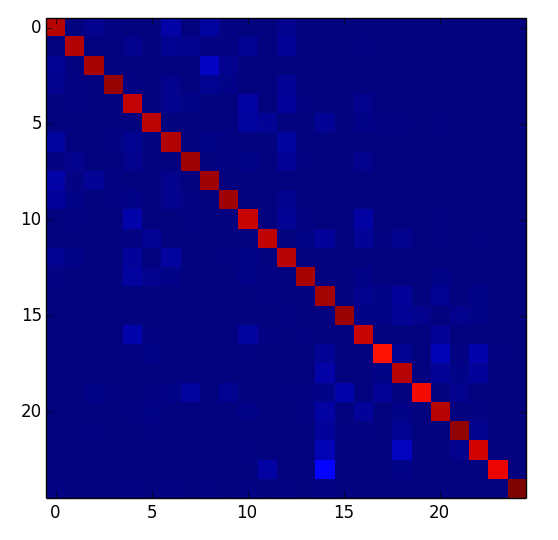
\includegraphics[width=0.5\textwidth]{trans-h.png}
   \caption{Initial Transition Matrix}
   \label{fig:transmath}
\end{figure}

\subsection{Evaluation}


What worked well? What didn't? Where did most of the errors occur?
What was our success rate? Did the results improve with HPSS?

Hey look a dinosaur.

\section{Conclusion and Future Work}

We have introduced a simple beat-synchronous automatic chord estimation model
and evaluated the effectiveness of HPSS as a preprocessing step.

Exploration of tuning, different hmm models (ex, better model for less frequent chords)

One preprocessing step that we have not considered in this paper is tuning. Because tuning pitch 
may differ between recordings, it may be necessary to consider different candidate chroma vectors. 
\cite{McVicar:00} suggests that tuning using Harte's tuning algorithm is a staple of most modern
algorithms. Some older papers such as \cite{Zenz:20} mention micro--tuning of the human voice as well 
as percussive sounds as sources of classification error, so tuning algorithms may be worth investigating 
as a future preprocessing stepin addition to HPSS. 

Each song in the Billboard dataset also includes key information. It is possible to use the HMM model to 
simultaneously estimate the chords and the key of an input audio file \cite{McVicar:00}, so a future
implementation may use this data to predict key information as well as chords.



\begin{thebibliography}{citations}

\bibitem{McVicar:00}
M. McVicar, et al.
"Automatic Chord Estimation for Audio: A Review of the State of the Art"
{\it IEEE/ACM Transactions on Audio, Speech, and Language Processing},
Vol.~22,No.~2, pp.~1-20, 2014.

\bibitem{Ueda:01}
Yushi Ueda, et al.
"HMM-Based Approach For Automatic Chord Detection Using Refined Acoustic Features''
{\it IEEE International Conference on Acoustics, Speech, and Signal Processing 2010},
pp.~5518--5521, 2010.

\bibitem{Varewyck:02}
Matthias Varewyck, et al.
"A Novel Chroma Representation of Polyphonic Music based on Multiple Pitch
Tracking Techniques''
{\it 16th ACM International Conference on Multimedia},
2008.

\bibitem{Lee:03}
Kyogu Lee
"Automatic Chord Recognition from Audio Using Enhanced Pitch Class Profile''
{\it Center for Computer Research in Music and Acoustics, Stanford},
2006.

\bibitem{Papadopoulus:04}
Hélène Papadopoulos and George Tzanetakis
"Modeling Chord and Key Structure With Markov Logic''
{\it 13th International Society for Music Information Retrieval Conference},
pp.~127-132, 2012.

\bibitem{Schorkhuber:05}
Christian Schorkhuber and Anssi Kalpuri
"Constant-Q Transform Toolbox for Music Processing" 
{\it 7th Sound and Music Computing Conference, Barcelona, Spain},
July 2010.

\bibitem{SciKit:06}
F. Pedregosa, et al.
"Scikit-learn: Machine Learning in Python"
{\it Journal of Machine Learning Research},
Vol.~12,pp.~2825-2830, 2011.

\bibitem{Burgoyne:07}
John Ashley Burgoyne, Jonathan Wild, and Ichiro Fujinaga
"An Expert Gound-Truth Set For Audio Chord Recognition and Music Analysis,"
{\it 12th International Society for Music Information Retrieval Conference},
pp.~633-638, 2011.

\bibitem{Burgoyne:08}
Nanzhu Jiang et al.
"Analyzing Chroma Feature Types for Automated Chord Recognition,"
{\it AES 42nd International Conference },
pp.~1-10, 2011.

\bibitem{Reed:09}
J.T. Reed, Yushi Ueda, S. Siniscalchi, Yuki Uchiyama, Shigeki Sagayama, C.-H. Lee
"Minimum Classification Error Training To Improve Isolated Chord Recognition"
{\it 10th International Society for Music Information Retrieval Conference (ISMIR 2009)},
pp.~609-614, 2009.

\bibitem{Mauch:10}
Matthias Mauch
"Automatic Chord Transcription from Audio Using Computation Models of Musical Context"
{\it School of Electronic Engineering and Computer Science, Queen Mary, University of London},
pp.~1-168, 2010.

\bibitem{FitzGerald:11}
Derry FitzGerald
"Harmonic/Percussive Separation Using Median Filtering"
{\it Proc\. of the 13th Int. Conference on Digital Audio Effects (DAFx-10), Graz, Austria, September 6-10, 2010},
pp.~1-4, 2010.

\bibitem{Blunsom:12}
Phil Blunsom
"Hidden Markov Models"
{\it Melbourne School of Engineering},
pp.~1-7, 2004.

\bibitem{Sumi:13}
Kouhei Sumi, KatsutoshiItoyama, Kazuyoshi Yoshii, Kazunori Komatani, Tetsuya Ogata, and Hiroshi G. Okuno
"Automatic Chord Recognition Based on Probabilistic Integration of Chord Transition and Bass Pitch Estimation"
{\it ISMIR 2008 - Session 1a - Harmony},
pp.~39-44, 2008.

\bibitem{Ryyananen:14}
Matti P. Ryyananen and Anssi P. Klapuri
"Automatic Transcription of Melody, Bass Line, and Chords in Polyphonic Music"
{\it Computer Music Journal, Volume 32, Number 3},
pp.~72-86, Fall 2008.

\bibitem{Lee:15}
Kyogu Lee and Malcolm Stanley
"Automatic Chord Recognition from Audio Using an HMM with Supervised Learning"
{\it AMCMM '06},
pp.~10-11, 2006.

\bibitem{Papadopoulus:16}
Hélène Papadopoulos and Geoffroy Peeters
"Large-Scale Study of Chord Estimation Algorithms Based on Chroma Representation and HMM"
{\it CBMI 2007},
pp.~53-60, 2007.

\bibitem{Salamon:17}
Justin Salamon and Emilia G{\'o}mez
"Melody Extraction from Polyphonic Music Signals using Pitch Contour Characteristics"
{\it IEEE Transactions on Audio, Speech and Language Processing},
pp.~1759-1770, 2012.

\bibitem{Papadopoulos:18}
Hélène Papadopoulos and Geoffroy Peeters
"Joint Estimation of Chords and Downbeats From an Audio Signal"
{\it IEEE Transactions on Audio, Speech and Language Processing, Vol. 19, No.1},
January 2011.

\bibitem{Ueda:19}
Yushi Ueda, Yuki Uchiyama, Takuya Nichimoto, Nobutaka Ono and Shigeki Sagayama
"HMM-Based Approach for Automatic Chord Detection Using Refined Acoustic Features"
{\it IEEE Transactions on Audio, Speech and Language Processing},
pp.~5518-5521, 2010.

\bibitem{Zenz:20}
Veronika Zenz and Andrea Rauber
"Automatic Chord Detection Incorporating Beat and Key Detection"
{\it IEEE International Conference on Signal Processing and Communicationg},
pp.~1175-1178, 2007.

\bibitem{Ellis:21}
Dan Ellis
"Supervised Chord Recognition for Music Audio in Matlab"
{\it LabROSA: Projects http://labrosa.ee.columbia.edu/projects/chords/},
2010. Last Accessed: Apr 17, 2014. 

\bibitem{Jiang:22}
Nanzhu Jiang, Peter Grosche, Verena Konz, and Meinard Muller.
"Analyzing Chroma Feature Types for Automated Chord Recognition"
{\it AES 42nd International Conference},
July 2011. 

\end{thebibliography}

\bibliography{ismir2013template}

\end{document}

